
\section{Results and Discussion}
\label{sec:results}
\noindent 
The results of our technique are discussed by means of application examples using real-world data sets and directions for future research are provided.
\begin{figure*}[t]
	\centering
	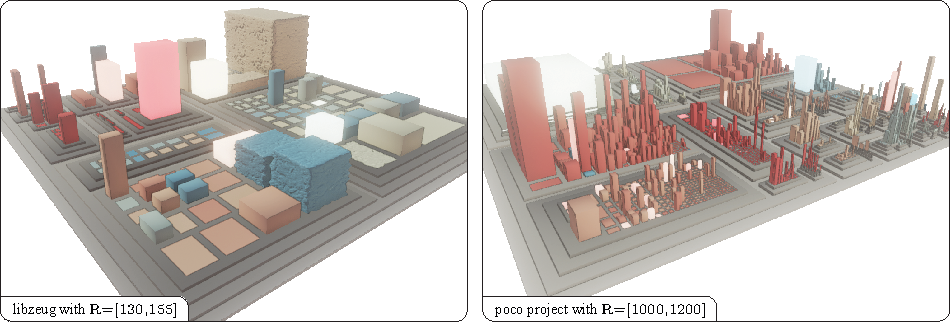
\includegraphics[width=1.0\textwidth]{results}
	\caption{
		Applications of the presented visualization technique using two real data sets using item-based natural phenomena as metaphors.
		The underlying software maps encode lines-of-code to item area, the mean nesting-level to height, and the number of file changes within the revision range to color. 
		Left: the trends of the McCabe metric is mapped into the range between a rough surface and glow. 
		Right: the inverted trend of the lines-of-code metric is mapped using the same metaphor.}
	\label{fig:results}
\end{figure*}
\Wrt to performance, the technique was tested using datasets of two software systems with different complexity, \ie different static structure components and number of revisions (\autoref{fig:results}):
\begin{table}[h]
	\centering
	\begin{tabular}{llll}
		\textbf{Data Set} & \textbf{\#Rev.} & \textbf{Rev. Range} & \textbf{max. \# Items} \\
		\midrule
		libzeug & 248 & [130,155] & 243 \\
		PocoProject & 2038 & [1000,1200] & 2635 \\
	\end{tabular}
\end{table}
\\
For each revision, the repository was downloaded, making it yet impractical for repositories containing binary files.
Gathering the revision data, computing and aggregating metric values for 72 software metrics for every revision of the master branch resulted in expensive preprocessing.
However, both projects can be rendered at interactive frame rates:
\begin{table}[h]
	\centering
	\begin{tabular}{llll}
		\textbf{Data Set} & \textbf{Metric Comp.} & \textbf{Aggr.} & \textbf{Rendering} \\
		\midrule
		libzeug     & appr. 04h & 04sec & 16ms \\
		PocoProject & appr. 48h & 17min & 43ms \\
	\end{tabular}
\end{table}

Our trend maps facilitate the depiction of metric changes over a revision range by extending software maps of a certain revision $x \in R$. 
Hence, a conceptual limitation of our approach, is that a trend map only shows trends for items which are still present at the respective revision $x$. 
A proper visualization of deleted or added system components within a software map is still subject to research.

Besides the static image approach for our trend maps, we have also tested several animated transitions for trend data of a revision range.
We tested linear interpolation and cubic interpolations using uniform, chordal, and centripetal catmull-rom splines \cite{Yuksel2009}. 
By additionally rendering these trend curves the user gets a familiar view to explore the trend data of a particular item or a group of items.
However, we found that using these trend curves to parametrize the natural phenomena during a transition animation overstrains the user's perception for complex real-world data sets, since there are too many change processes visualized simultaneously.

The presented approach can be used to facilitate overview of hot spots in software maps according to the information \enquote{seeking mantra: overview first, zoom and filter, then details-on-demand} \cite{Shneiderman1996}.
Especially effects such as glow seem to support pre-attentive processing and can be used for
highlighting purposes, but in contrast to rust or shiny effects, it alters the item's color mapping significantly and complicates the perception of shape. 
However, the perception of surface effects such as rust or corrosion depends on items' screen sizes.
Also, when depicting larger revision ranges the number of affected items and regions tend to cause cluttering and context-based metaphors (\eg fire) comprising large regions-of-interest sometimes cause occlusion. 

\paragraph*{Future Work}
We plan to focus our research on evaluation and adjustment of the visual metaphors by conducting a comprehensive user study. 
\Wrt this, research on how certain effects (\eg fire or thunderstorms) are able to emotionalize.
Furthermore, care has to be taken on how many natural phenomena implemented can be applied simultaneously and still be perceived and distinguished by users (\autoref{fig:additional-result}).
Another topic for future work can be to evaluate different forecasting methods for software metrics and directly map them to metaphors commonly used in daily weather forecasting visualizations.
To allow for natural phenomena to be used on larger data sets, level-of-detail (LoD) compliance of the presented techniques has to be evaluated, \eg for surface appearances, since fine surface details are hard to perceive if the virtual camera is far away from a region-of-interest.

\begin{figure}[b]
	\centering
	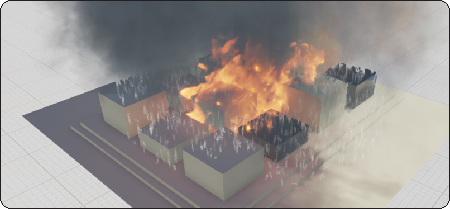
\includegraphics[width=1.0\linewidth]{additional-result}
	\caption{Superposition of multiple natural phenomena.}
	\label{fig:additional-result}
\end{figure}